%% ====================================================================
%%  Chapter 4 — How We Measure: Metrics and Evaluation
%% ====================================================================
\chapter{How We Measure: Metrics and Evaluation}
\label{ch:eval}

You cannot interpret a single result in Chapter~\ref{ch:arch} without first understanding how the
numbers are produced. This chapter defines the error metric, explains how a whole \emph{distribution}
of errors is summarized (and a quantization trap to avoid), describes the corruptions used to probe
robustness, and clarifies the two very different cross-session protocols and the efficiency numbers.

\section{The localization error metric}
\label{sec:eval:error}

Every model outputs a heatmap; the prediction is the \textbf{peak} (argmax) of that heatmap. The error
for one sample is the physical distance between the predicted peak and the ground-truth peak:
\[
  e \;=\; 0.1 \times \big\lVert \arg\max(\hat{y}) - \arg\max(y) \big\rVert_2 ,
\]
i.e.\ the Euclidean pixel distance, scaled by the $0.1$\,m-per-pixel resolution of the grid. So an
error of $0.7$ means the predicted location was $0.7$\,m from the truth. Simple, physical, and the
only metric that matters for a localization system.

\section{Summarizing a distribution: median, P90, P99, mean}
\label{sec:eval:stats}

A model produces one error per test sample ---thousands of them. We summarize that distribution with
four numbers, each answering a different question:
\begin{description}[leftmargin=1.6cm,style=nextline,nosep]
  \item[Median] The typical case: half of predictions are better than this, half worse. It is robust
  to a few wild outliers, which is why it is the headline accuracy number.
  \item[P90 (90th percentile)] $90\%$ of predictions are within this distance. It describes the
  \emph{tail} ---how bad the routine-but-unlucky cases get.
  \item[P99 (99th percentile)] The near-worst case; dominated by a handful of genuinely ambiguous
  locations. Expect it to be noisy from seed to seed.
  \item[Mean] The average. Unlike the median, it \emph{is} sensitive to large errors, so a gap between
  mean and median signals a heavy tail.
\end{description}

\begin{defensetip}
Know \emph{why} we report all four. The median alone can be misleading (next section); the mean
exposes heavy tails; P90/P99 describe worst-case behavior that matters for a deployed system. When a
table shows two models with the same median but different means, the one with the lower mean has the
lighter tail ---a real, if subtle, advantage.
\end{defensetip}

\section{Reading a CDF}
\label{sec:eval:cdf}

The \textbf{cumulative distribution function} (CDF) of the error plots, for every distance $d$ on the
$x$-axis, the \emph{fraction of predictions with error $\le d$} on the $y$-axis. It is the most honest
single picture of a model's accuracy because it shows the entire distribution at once, not a single
percentile.
\begin{itemize}[leftmargin=1.4em,nosep]
  \item A curve that rises \emph{up and to the left} is better (more predictions are accurate at
  smaller distances).
  \item The height at a given $x$ is ``what fraction of the time am I within $x$ meters?''
  \item The median is where the curve crosses $0.5$; P90 is where it crosses $0.9$.
\end{itemize}
Figure~\ref{fig:eval:cdf} is exactly this plot for our in-distribution results: the MobileNetV2-UNet
curve sits above the plain MobileNetV2 across the whole range, while TinyCNN never even reaches the
$0.8$ level within 3\,m ---a one-glance summary of the capacity story.

\begin{figure}[H]
\centering
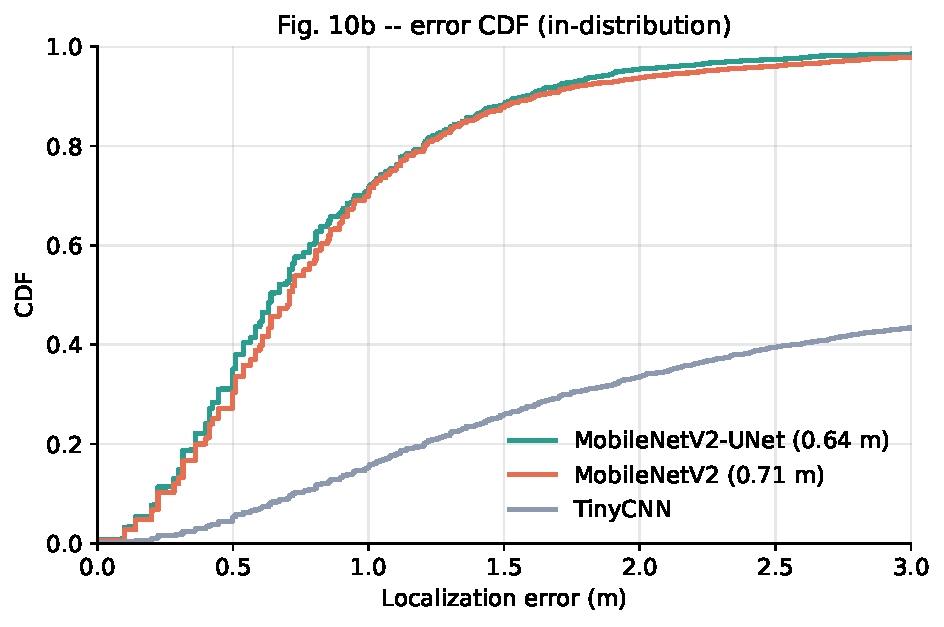
\includegraphics[width=0.74\linewidth]{cdf_fig10b}
\caption{In-distribution error CDF. Read it as: at each distance on the $x$-axis, what fraction of
predictions are at least that accurate ($y$-axis). The MobileNetV2-UNet dominates (up and to the
left); TinyCNN, starved of capacity, never reaches the $0.8$ level within 3\,m.}
\label{fig:eval:cdf}
\end{figure}

\section{The pixel-quantization gotcha}
\label{sec:eval:quant}

Here is a trap that the thesis is careful about and a committee may probe. Because the error is a
\emph{pixel} distance scaled by $0.1$, and pixel offsets are integers, the achievable error values are
\emph{quantized}: they can only be multiples of $0.1\sqrt{n}$ for integer $n$ (since
$\sqrt{\Delta x^2 + \Delta y^2}$ with integer $\Delta x,\Delta y$ takes only discrete values
$0,\,1,\,\sqrt2,\,2,\,\sqrt5,\dots$). One consequence is decisive:

\begin{keyidea}
Two models can report the \emph{identical} median (e.g.\ several of ours sit exactly at $0.707$ or
$0.640$\,m) yet have genuinely different error \emph{distributions}. An identical median is sometimes
a quantization artifact, \emph{not} evidence that the models are equally good. This is precisely why
the thesis reports the mean, the percentiles, and the full CDF alongside the median ---and why you
should never argue a result from the median alone.
\end{keyidea}

\section{Robustness corruptions}
\label{sec:eval:corruptions}

Robustness is measured by \emph{corrupting the CSI input at test time only} ---the models are
\textbf{not} retrained ---and re-measuring the error. Each corruption simulates a real-world failure:
\begin{description}[leftmargin=2.0cm,style=nextline,nosep]
  \item[AP dropout] Zero out one AP's channel, either a specific AP or a random one (and random
  2-AP dropout). Simulates an access point failing or going out of range.
  \item[Gaussian noise $\sigma\in\{0.1,0.2\}$] Add random noise to the CSI. Simulates interference and
  low signal-to-noise conditions.
  \item[Global attenuation $0.5\times$] Halve the whole signal. Simulates overall signal weakening.
  \item[Single-AP attenuation $0.3\times$] Drop one AP's strength to $30\%$. Simulates one weak or
  distant AP.
  \item[Blur ($5\times5$, $\sigma{=}1$)] Gaussian-blur the CSI heatmap. Simulates loss of spatial
  sharpness / lower effective bandwidth.
\end{description}
Testing without retraining is the strict choice: it measures how a \emph{deployed} model copes with
conditions it never saw, rather than how well it can be trained to anticipate them. (Training-time
corruption augmentation is left to future work.)

\section{Cross-session protocols: the fair one and the ablation}
\label{sec:eval:crosssession}

``Cross-session'' means testing in a different data-collection session than you trained on ---the
realistic case where the environment changes over time. The thesis runs \emph{two} protocols, and
keeping them straight is essential because only one is a fair comparison to DLoc.

\begin{description}[leftmargin=1.6em,style=nextline,nosep]
  \item[Leave-one-session-out (LOSO) --- the fair comparison.] Three folds; each fold holds out one
  August session and trains on the remaining setups, then tests on the held-out session. We run the
  MobileNetV2-UNet over three random seeds per fold. This \emph{exactly matches the protocol used to
  report the published DLoc numbers}, so the comparison in Section~\ref{ch:arch} is apples-to-apples.
  Because re-distilling would require retraining a teacher per fold, the LOSO models are
  \textbf{standalone only}.
  \item[Zero-shot stress test --- an internal ablation.] Train on \emph{only} the two July sessions
  and evaluate on the August sessions. This deliberately uses less training data and is \textbf{not} a
  fair DLoc comparison; it exists to compare \emph{our own} architectures and the effect of
  distillation against each other under a harder shift.
\end{description}

\begin{defensetip}
If a committee member compares our cross-session numbers to DLoc, make sure they are looking at the
\textbf{LOSO} table (mean $0.930$\,m vs DLoc $0.86$\,m), not the zero-shot table. Conflating the two
understates the model. The zero-shot numbers answer a different question (``does distillation help
under a bigger shift?'' ---yes, but only on the hardest fold).
\end{defensetip}

\section{The session difficulty hierarchy}
\label{sec:eval:sessions}

The WILD dataset has five sessions (Table~\ref{tab:eval:sessions}). They are not equally hard: errors
rise monotonically from the furniture sessions to the reflector session, a property of the
\emph{environment}, not of any model. The aluminum-reflector session is hardest because it injects
strong \emph{specular multipath} ---mirror-like reflections that create convincing ``phantom''
locations.

\begin{table}[H]
\centering
\caption{The five WILD collection sessions (Jacobs Hall, UC San Diego, 4 APs).}
\label{tab:eval:sessions}
\begin{tabular}{@{}llrl@{}}
\toprule
\textbf{Session} & \textbf{Tag} & \textbf{Samples} & \textbf{Condition} \\
\midrule
1 & \code{jacobs\_Jul28}        & ---     & training (reference conditions) \\
2 & \code{jacobs\_Jul28\_2}     & 4{,}260$^\dagger$ & in-distribution test (1\,h later, identical) \\
3 & \code{jacobs\_Aug16\_1}     & 11{,}201 & furniture rearrangement \\
4 & \code{jacobs\_Aug16\_3}     & 8{,}754  & different furniture configuration \\
5 & \code{jacobs\_Aug16\_4\_ref}& 5{,}486  & aluminum reflector (specular multipath) \\
\bottomrule
\end{tabular}

\vspace{0.3em}
{\footnotesize $^\dagger$ Held-out test split; Sessions~1+2 together provide 17{,}574 training
samples. Sessions 3--5 were collected three weeks later with deliberate environmental changes.}
\end{table}

\section{Computational efficiency metrics}
\label{sec:eval:efficiency}

Finally, deployment cost is measured four ways (reported in the thesis's efficiency table):
\begin{description}[leftmargin=1.8cm,style=nextline,nosep]
  \item[Parameters] The model's memory footprint ---how much storage/RAM the weights need.
  \item[FLOPs] Floating-point operations for one forward pass (batch size 1, dummy input). The
  compute cost per prediction.
  \item[CPU latency] Wall-clock time for one prediction on a CPU ---\textbf{the number that matters
  most for edge deployment}, since most gateways and APs have no GPU.
  \item[GPU latency] Wall-clock time on a GPU, for completeness.
\end{description}
The punchline you will need cold: the MobileNetV2-UNet runs in $27.2$\,ms on CPU and $1.45$\,GFLOPs,
versus DLoc's $270.9$\,ms and $81.06$\,GFLOPs ---a $10\times$ latency and $56\times$ compute reduction
at \emph{better} accuracy. That combination is the whole case for edge deployment.
